\documentclass[parskip=full]{scrartcl}
\usepackage[T1]{fontenc}
\usepackage[utf8]{inputenc}
\usepackage[ngerman]{babel}
\usepackage{hyperref}
\hypersetup{
	pdftitle={PSE: Blockchain-basiertes E-Voting - Implementierungsbericht},%
	,%
}
\usepackage{graphicx}
\usepackage{csquotes}
\usepackage[nonumberlist]{glossaries}
\usepackage{enumitem}
\usepackage{xcolor}
\usepackage{svg}
\usepackage[section]{placeins}

\makeatletter
\AtBeginDocument{%
	\expandafter\renewcommand\expandafter\subsection\expandafter{%
		\expandafter\@fb@secFB\subsection
	}%
}
\makeatother
\makeatletter
\AtBeginDocument{%
	\expandafter\renewcommand\expandafter\subsubsection\expandafter{%
		\expandafter\@fb@secFB\subsubsection
	}%
}
\makeatother

\addto\extrasngerman{\def\figureautorefname{Abb.}}
\newcommand{\textitx}[1]{\mbox{\textit{#1}}}
\newcommand{\fakeparagraph}[1]{\textbf{#1}}
%\renewcommand{\includesvg}[1][1]{}


\title{
	PSE:Blockchain-basiertes E-Voting \\
	Implementierungsbericht
}
\author{Tim Fröhlich, Achim Kriso, Philipp Schaback, David Schuldes, Artem Vasilev\\ Phasenverantwortlicher: Philipp Schaback}



\begin{document}
\clearpage
\maketitle
\pagenumbering{gobble}
\newpage

\tableofcontents
\newpage
\pagenumbering{arabic}

\section{Einleitung}
Dieses Dokument beschreibt die Ergebnisse der Implementierungsphase, die
im Rahmen des Moduls Praxis der Softwareentwicklung (PSE) am Lehrstuhl „Anwendungsorientierte formale Verifikation" von Prof. Dr. Beckert am Karlsruher Institut für
Technologie entstanden sind.
Implementiert wurde die im Pflichtenheft vorgegebene und in der Entwurfsphase entworfene Software "Blockchain-basiertes Evoting".


\section{Zeitablauf}
Um einen schnellen und erfolgreichen Abschluss der Implementierung zu begünstigen, begann diese bereits Ende Juni.
Die im Entwurfsdokument angegebene Zeiteinschätzung wurde hierbei weitestgehend eingehalten, in vorteilhaft gestauchter Version (siehe \autoref{fig:gantt}).
\begin{figure}[h!]
	\centering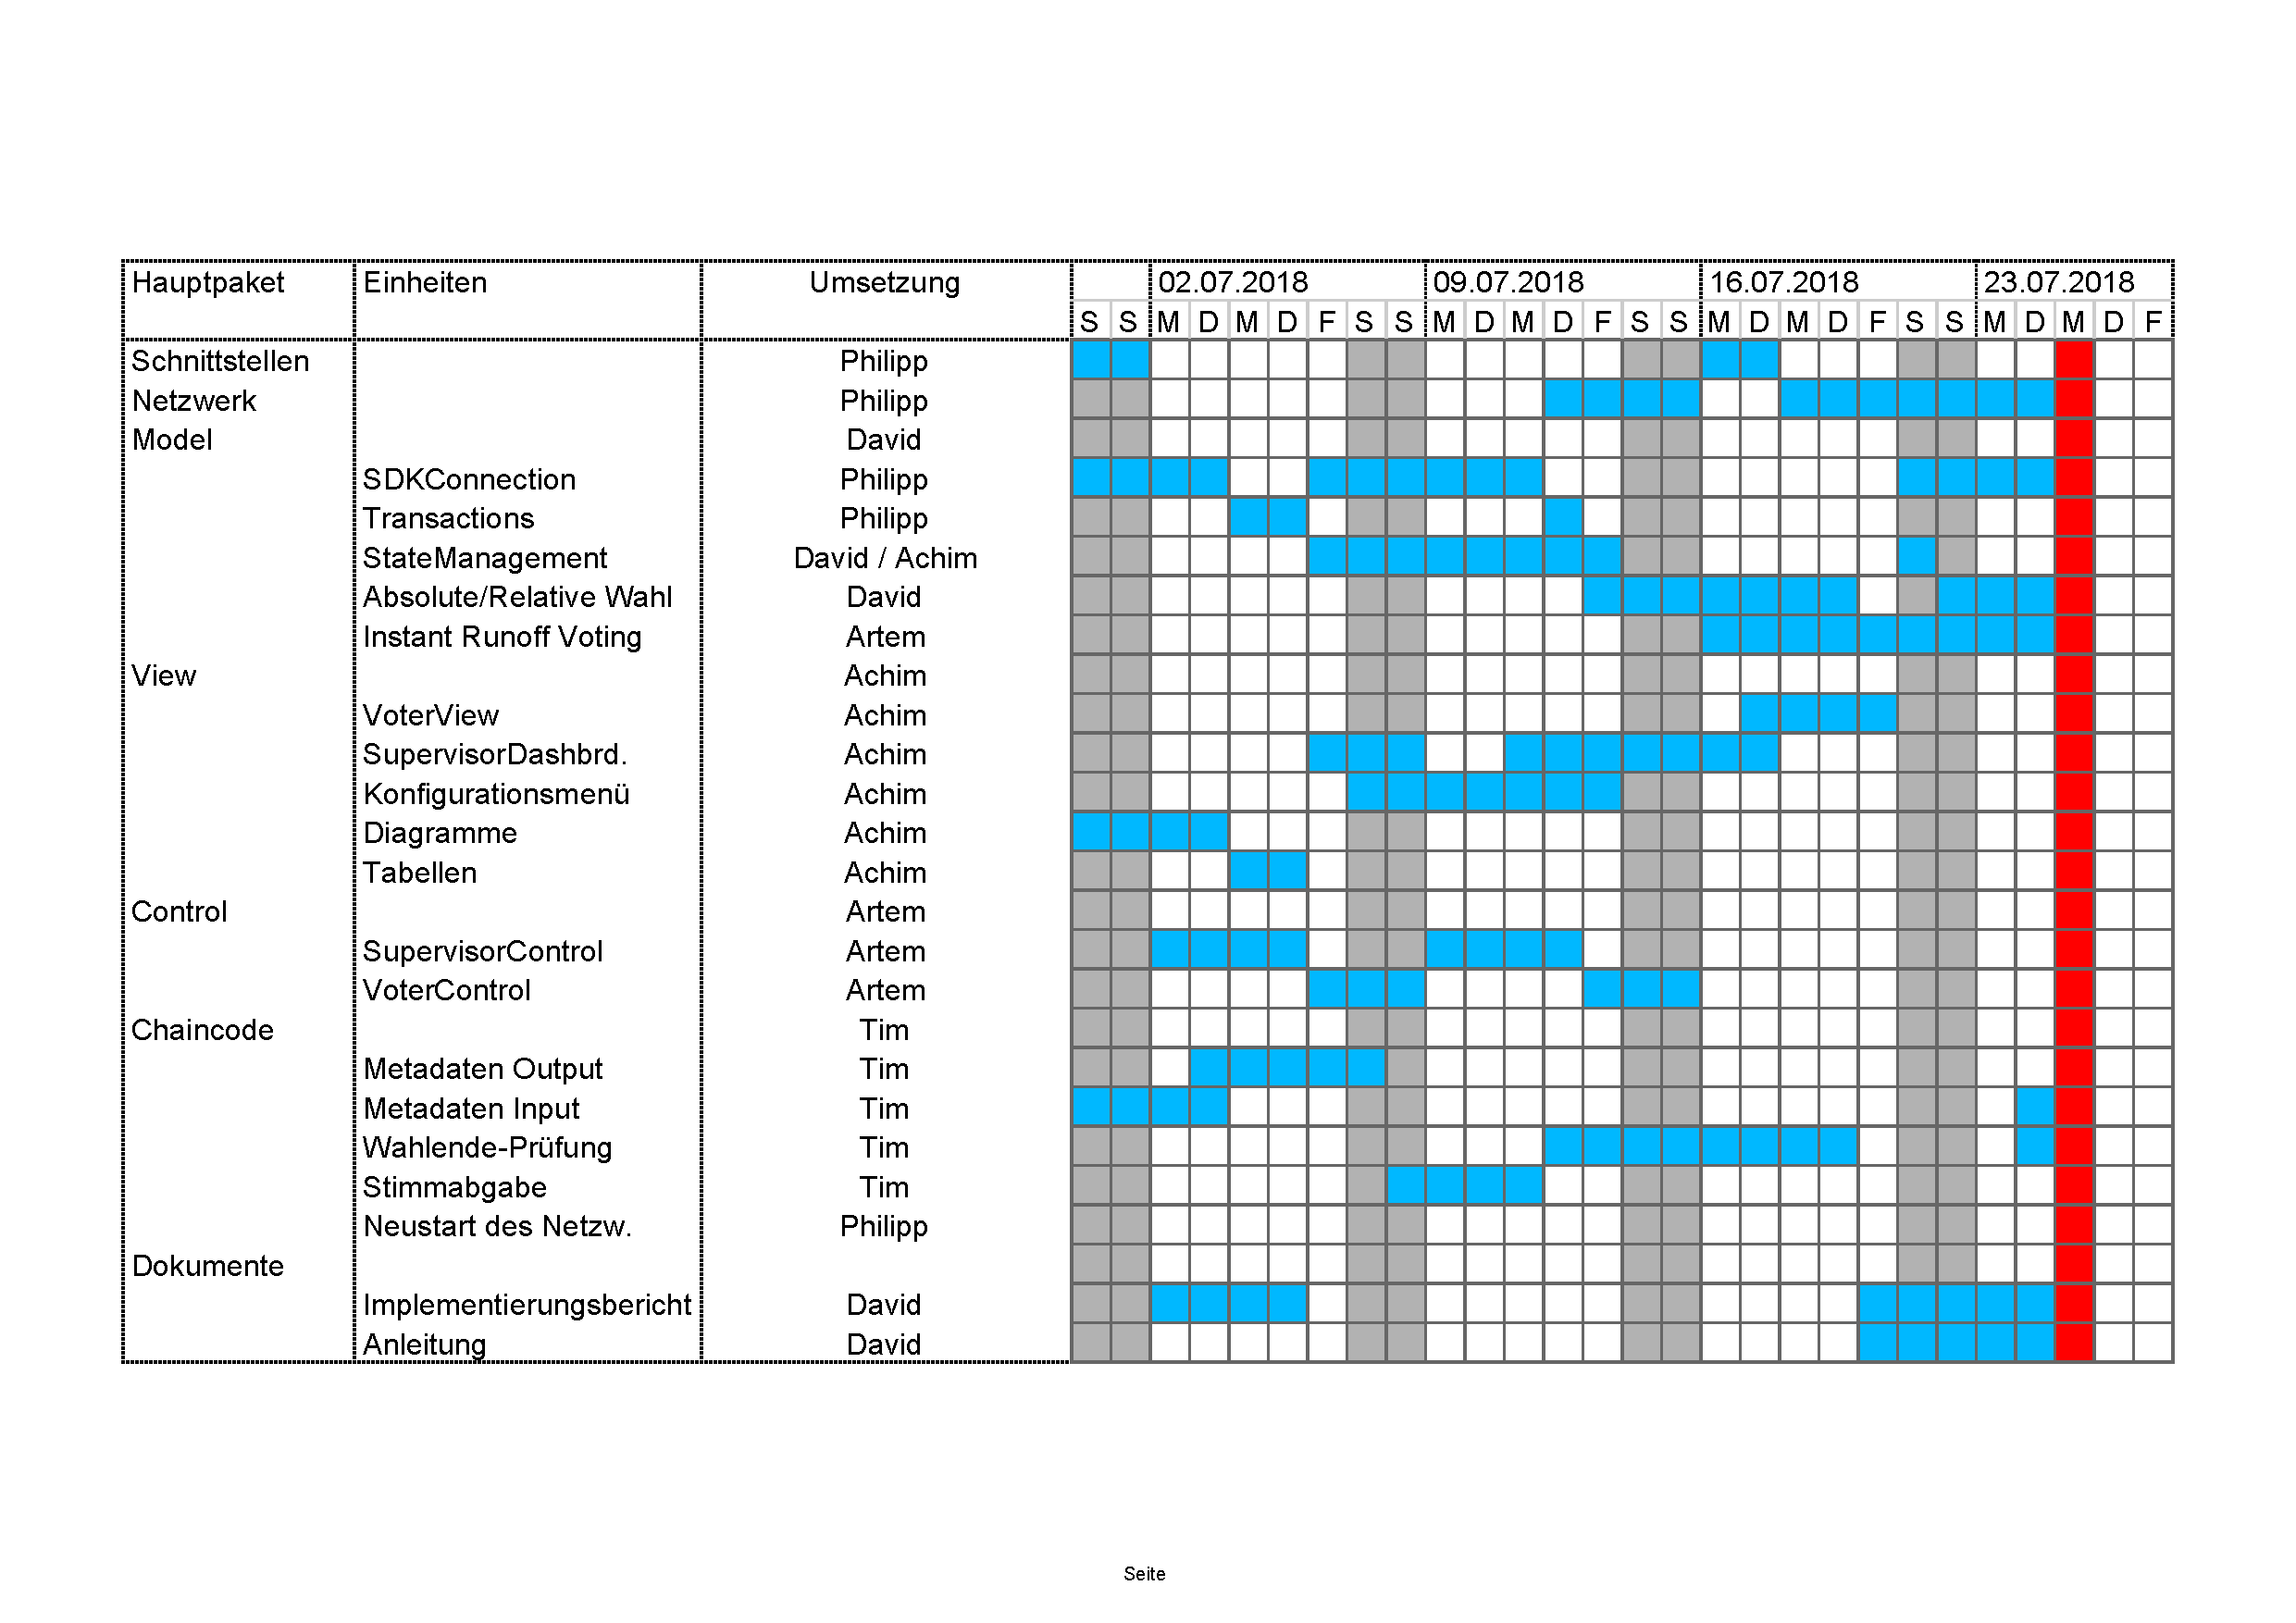
\includegraphics[width=\textwidth]{pictures/Gantt.pdf}
	\caption{Gantt-Diagramm (unvollständig)}
	\label{fig:gantt}
\end{figure}


\section{Umsetzung der funktionalen Anforderungen}

\subsection{Musskriterien}
Alle im Pflichtenheft festgelegten Musskriterien werden durch die Implementierung umgesetzt.

\subsection{Sollkriterien}
Die Sollkriterien wurden alle bis auf eines erfüllt:
\textit{S3: Dynamische Peerverbindung}\\
Teil des Sicherheitsmodells von Hyperledger Fabric ist, dass ein Client Verbindungen zu mehreren Peers herstellt, das Kriterium sieht aber nur die Verbindung zu einem Peer vor.
Somit wäre eine Umsetzung von S3 der korrekten und sicheren Wahl entgegenstehend. Dennoch ermöglichen wir es, einzelne Peers mittels der Konfigurationsdatei auszuschließen.  

\subsection{Kannkriterien}
Alle Kannkriterien, ausgenommen von \textit{K2: Geheime Wahlen} wurden umgesetzt. Die Implementierung von geheimen Wahlen zeigte sich bei unseren Nachforschungen als besonders aufwändig, da der Ledger grundsätzlich \enquote{by design} öffentlich ist. Mögliche Strategien wie das Verschlüsseln der Stimmen beim Wähler und späteres Entschlüsseln wurden als Lösung in Betracht gezogen. Selbst hiermit erweist sich die Umsetzung als problematisch, da die Auswertung der Stimmen vom Klienten in die Smart Contracts verlegt werden müsste, um wahrhaft geheim zu sein. Eine solche Auszählung wird durch die verschiedenen Wahlsysteme und deren unterschiedliche Auszählungsverfahren zusätzlich erschwert. Es wäre nur schwer nachzuverfolgen, welcher Chaincode tatsächlich eingesetzt wird. Im Gegensatz dazu könnte beispielsweise der Source Code des Klienten offengelegt werden und ein solcher Wähler könnte nachvollziehen, dass die Auswertung korrekt vonstatten ging.

\section{Umsetzung der nichtfunktionalen-Anforderungen}

Alle im Pflichtenheft definierten, nicht-funktionale Anforderung wurden erfüllt. Im Folgenden sind sie in die Kategorien Zeitverhalten und Benutzerfreundlichkeit unterteilt.

\subsection{Zeitverhalten}

\begin{itemize}
	\item Die Stimmabgabe eines Wählers dauert vorraussichtlich nicht länger als 5 Minuten. Diese Anforderung wurde bei allen, die Stimmabgabe betreffenden, ausgeführten Testfällen erfüllt.
	\item Die grafische Benutzeroberfläche reagiert sofort bei Interaktions des Benutzers. Diese Anforderung wurde bei allen bisher ausgeführten Testfällen, welche die Benutzeroberfläche betreffen erfüllt.
	\item Die Auswertung einer Wahl nimmt bei höchstens 10000 abgegebenen Stimmen vorraussichtlich nicht mehr als 5 Minuten in Anspruch. Diese Anforderung konnte bisher nicht getestet werden, aufgrund von einem bekannten Problem (siehe \autoref{sect:problem}) bei der Stimmabgabe mehrerer Wähler.
\end{itemize}

\subsection{Benutzerfreundlichkeit}
\begin{itemize}
	\item Im Pflichtenheft wurde definiert, dass die Benutzung der Software erfordert keine besonderen Vorkenntnisse, so dass sie auch Benutzer mit geringen Computerkenntnissen verwenden können. Die Wähler-und Wahlleiter-Benutzeroberfläche wurde so implementiert, dass die Interaktion mit der Software intuitiv vonstatten gehen kann.
\end{itemize}

\section{Produktleistungen}
Im Pflichtenheft wurde definiert, dass erfolgreich abgegebene Stimmen unverfälscht in die Auswertung der Wahl eingehen und genau einmal gewertet werden. Es soll nicht möglich, Stimmabgaben zu verfälschen und somit das Ergebnis der Wahlauswertung zu manipulieren.
Diese Anforderungen werden von den im Pflichtenheft definierten Muss-Kriterien abgedeckt, diese sind wiederum vollständig bei der Implementierung umgesetzt werden. Damit ist ebenso sichergestellt, dass Stimmen unverfälscht in die Wahl eingehen und es nicht möglich ist, eine Wahl dadurch zu manipulieren.

		
\section{Umsetzung von Entwurfsentscheidungen}
\subsection{Model-View-Control Architektur}
Bei der Implementierung wurden alle Pakete und Schnittstellen unter Einhaltung der in der in der Entwurfsphase modellierten Model-View-Control Architektur implementiert. Die Architektur sorgt für eine hohe Modularität der einzelnen Komponenten. Sie können problemlos unter Einhaltung der nach außen angebotenen Schnittstellen ausgetauscht und erweitert werden. 

\subsection{Strategie-Entwurfsmuster}
Im StateManagement-Paket wurde das Strategie-Entwurfsmuster in den Klassen IRVVoting, AbsoluteMajorityVoting und RelativeMajorityVoting bei der Implementierung von determineWinner() benutzt.
Das Auszählungverfahren der Stimmen ist abhängig von der festgelegten Wahlform und erfolgt mithilfe der determineWinner()-Methode, die jeweils in den zuvor genannten Klassen implementiert ist.
determineWinner() führt den Algorithmus zur Wahlauswertung aus. Deswegen finden sich in den Klassen IRVVotingSystem, RelativeMajorityVotingSystem und AbsoluteMajorityVotingSystem jeweils unterschiedliche Implementierungen der benötigten Variante des Auszählungsalgorithmus.
Der Vorteil hierbei ist, dass der Auszählungsalgorithmus modular gekapselt und austauschbar ist. Es können weitere Auszählungsverfahren hinzugefügt werden, ohne dass zusätzliche Anpassungen in anderen Klassen vorgenommen werden müssen.

\subsection{Fassaden-Entwurfsmuster}
Das Fassaden-Entwurfsmuster wurde bei der Implementierung der Schnittstellen ViewToControl, ControlToView, ControlToModel und ViewToModel benutzt. Die Schnittstellen delegieren die Funktionalitäten an Ihre jeweiligen Subsysteme (Controo, Model und View) und sorgen dafür, dass eine lose Kopplung zwischen den Subsystemen besteht.
Das hat den Vorteil, dass die Kommunikation zwischen den Paketen nur durch die Methoden in den Schnittstellen erfolgt und die Subsysteme beliebig ausgetauscht und erweitert werden können, solange sie die Schnittstellen implementieren.

\subsection{Schablonenmethode-Entwurfsmuster}
Das Schablonenmethoden-Entwurfsmuster wurde im Paket Transactions bei der Implementierung der Klassen QueryTransaction und InvokeTransaction benutzt.
Die beiden Klassen besitzen jeweils die abstrakten Methoden query() bzw. invoke() --hier brauche ich noch technischen Hintergrund

\subsection{Beobachter-Entwurfsmuster}
Das Beobachter-Entwurfsmuster wurde bei der Implementierung des ElectionListener-Interfaces und der SDKEventListenerImpl-Klasse im Model-Paket benutzt. Der Listener benachrichtigt die Supervisor-bzw. VoterGUI darüber, ob die Wahl beendet oder noch aktiv ist. Dadurch wird die SUpervisor- bzw. VoterGUI direkt über das Wahlende benachrichtigt. Andernfalls müsste eine periodische Anfrage an das Netzwerk gesendet werden, um zu ermitteln, ob die Wahl aktiv ist oder nicht.

\section{Änderungen zum Entwurf}
\paragraph{Interfaces}
Die Argumente und Rückgabetypen aller Interfaces wurden zu Beginn der Implementierung besser aufeinander abgestimmt um Inkonsistenzen zu entfernen.

\subsection{SDKConnection}

\paragraph{SDKConnectionImpl}
Die Klasse \textit{SDKConnectionImpl} wurde von einem normalen Konstruktor auf eine Fabrikmethode (\textit{getInstance()}) umgestellt, da Java \textit{super} als ersten Aufruf im Konstruktor erzwingt, und dies nicht mit dem Entwurf vereinbar war.

\subsection{View}

\paragraph{InformationPanel}
In der SupervisorView als auch in der VoterView werden die allgemeinen Informationen einer Wahl in einem \textit{JPanel} angezeigt. Um die Konfiguration dieses \textit{JPanel} zu vermeiden wurde die Implementierung in die \textit{InformationPanel} Klasse ausgelagert, welche von der SupervisorView und der \textit{VoterView} verwendet wird.

\paragraph{ImagePanel-Klasse}
Im Paket Components wurde die ImagePanel Klasse hizugefügt. Sie ermöglicht die Darstellung des Logos der Software auf der Benutzeroberfläche für Wähler und Wahlleiter. 

\paragraph{SupervisorVSComponentManager}
In \textit{SupervisorVSComponentManager} wurde die Methode \textit{updateResults()} hinzugefügt, um die von \textit{SupervisorVSComponentManager} generierten Komponenten mit neueren Ergebnisse zu aktualisieren.

\paragraph{ActiveListener-Klasse}
Die \textit{VerticalTabs} Klasse benachrichtigt ihre enthaltenen \textit{JPanel}, mithilfe von der neuen Klasse \textit{ActiveListener}, welcher Tab gerade ausgewählt wurde. Diese Funktionalität wird benötigt damit die Konfiguration überprüft werden kann, wenn der Benutzer sich die Übersicht seiner Konfiguration darstellen lässt. 

\paragraph{GapExtension-Klasse}
Es wurde die \textit{GapExtension}-Klasse hinzugefügt. Diese Klasse ermöglicht es, in Tabellen eine Lücke einzufügen. Das wurde für nötig befunden, denn es erwies sich als optisch ansprechender, die Tabellen an der Benutzeroberfläche mit einer Umrandung darzustellen.

\paragraph{ListExtensions-Konstruktor}
Um einheitliche Schriftarten in der View zu ermöglichen, nehmen die \textit{ListExtension}-Konstruktoren eine Instanz von \textit{Font}.
\\
\\
Außerdem bekamen \textit{TextExtension}, \textit{TextFieldExtension} und \textit{DescriptionExtension} eine \textit{setText()} Methode, \textit{TextFieldExtension} und \textit{DescriptionExtension} eine \textit{setEditable()} Methode, mit welchen sich das Wahlformular des Wählers gleichzeitig zum Anzeigen seiner Stimme verwenden lässt.

\paragraph{setBorder()-Methode}
Diese Klasse BasicList wurde um die \textit{setBorder()}-Setter erweitert. Mit dieser Methode kann man den Rand einer Liste verändern und (wichtig für unseren Zweck) deaktivieren. Der Grund für die Implementierung dieser Klasse ist, dass die Darstellung einer Listen in der Benutzeroberfläche mit Rand unübersichtlicher erscheint und einer nutzerfreundlichen Bedienbarkeit entgegensteht.

\subsection{Model}
\paragraph{StateManagement-Paket}
Die Klassen Candidate, Vote und SingularVote, die in der Implementierung modelliert wurden, sind in der Implementierung des StateManagement-Paketes nicht umgesetzt worden.

Diese Klassen sollten die Informationen über die erfolgreich abgegebenen Stimmen speichern und für die Auszählung der Stimmen, welche in einer VotingSystem Klasse erfolgt, bereitstellen.
Da die Informationen nur von der VotingSystem-Klasse benötigt werden
stellte es sich als effizienter heraus, die Informationen über die abgegebenen Stimmen direkt in der VotingSystem-Klasse zu speichern.

\paragraph{hasVoted()-Methode}
Im Model-Paket wurde im VoterControlToModel-Interface eine zusätzliche Methode hasVoted() implementiert. Sie überprüft, ob ein Wähler bereits seine Stimme abgegeben hat und ist nötig, weil die Wähler-GUI einem Wähler, der noch nicht gewählt hat, die Oberfläche zur Kandidatenauswahl anzeigt. Hat der Wähler bereits gewählt, wird ihm der Wartebildschirm angezeigt.

\subsection{Chaincode}
\paragraph{initStatusQuery()-Methode}
Im Chaincode-Paket wurde eine zusätzliche Methode InitStatusQuery() implementiert, um zu prüfen, ob eine Wahl auf der Blockchain initialisiert wurde. Die Methode wird benötigt, damit Supervisor- und VoterGUI ermitteln können, ob sie die Daten der Wahl zur Anzeige auf der Benutzeroberfläche von der Blockchain anfordern können. Das ist erst möglich, sobald eine Wahl auf der Blockchain initialisiert wurde.

\subsection{Control}
\paragraph{isElectionInitialized()-Methode}
Im ControlToModel-Interface wurde die Methode isElectionInitialized() hinzugefügt. Sie wird benötigt, damit ausgehend vom Control-Paket die initStatusQuery()-Methode über die ControlToModel-Schnittstelle aufzurufen.

\subsection{Utils}
\paragraph{ConfigResourceBundle-Klasse}
Im Utils-Paket wurde eine Klasse ConfigResourceBundle hinzugefügt. Sie ermöglicht, dass Software-externe Config-Dateien in die Software geladen werden können. Das ist nötig, da ansonsten nur auf in der .jar-Datei mitgelieferte Config-Dateien zugegriffen werden kann.


\section{Bekannte Probleme} 
\label{sect:problem}
Nachdem ein Wähler seine Stimme erfolgreich abgegeben hat wird jedem Wähler, auch solchen, die noch keine Stimme abgegeben haben, der Wartebildschirm des Wählers der als erster seine Stimme abgegeben hat, angezeigt.
Dieses Verhalten ist erst eineinhalb Tage vor Ende der Implementierungsphase beim Integrationstest der Software aufgefallen, da alle Testfälle, welche die Funktionalität der einzelnen Pakete testeten, ohne Komplikationen verlaufen sind.

\end{document}

